%%%%%%%%%%%%%%%%%%%%%%% file template.tex %%%%%%%%%%%%%%%%%%%%%%%%%
%
% This is a general template file for the LaTeX package SVJour3
% for Springer journals.          Springer Heidelberg 2010/09/16
%
% Copy it to a new file with a new name and use it as the basis
% for your article. Delete % signs as needed.
%
% This template includes a few options for different layouts and
% content for various journals. Please consult a previous issue of
% your journal as needed.
%
%%%%%%%%%%%%%%%%%%%%%%%%%%%%%%%%%%%%%%%%%%%%%%%%%%%%%%%%%%%%%%%%%%%
%
\RequirePackage{fix-cm}
%
%\documentclass{svjour3}                     % onecolumn (standard format)
\documentclass[smallcondensed]{svjour3}     % onecolumn (ditto)
%\documentclass[smallextended]{svjour3}      % onecolumn (second format)
%\documentclass[twocolumn]{svjour3}          % twocolumn
%
\smartqed  % flush right qed marks, e.g. at end of proof
%
\usepackage{graphicx}
%
% \usepackage{mathptmx}      % use Times fonts if available on your TeX system
%
% insert here the call for the packages your document requires
%\usepackage{latexsym}
% etc.
%
% please place your own definitions here and don't use \def but
% \newcommand{}{}
%
% Insert the name of "your journal" with
\journalname{AStA Advances in Statistical Analysis}

% Own Packages and newcommands
\usepackage{amsmath, amssymb}
\setlength{\parindent}{0pt} % remove indentation before every paragraph
\usepackage{booktabs}
\usepackage{multirow}
\usepackage{float} % to force figure placement
\usepackage[usenames, dvipsnames]{color}
% \usepackage[backend=bibtex,
%             style=nature,
%             citestyle=authoryear]{biblatex}
% \addbibresource{bauer_2018.bib}
\usepackage{natbib}
\bibliographystyle{smj}
\newcommand{\T}{\mathrm{\scriptscriptstyle T}}
\newcommand{\red}[1]{\textcolor{red}{#1}}



\begin{document}
\title{KOALA: Estimating coalition probabilities in multi-party electoral systems%\thanks{Grants or other notes
%about the article that should go on the front page should be
%placed here. General acknowledgments should be placed at the end of the article.}
}
\subtitle{Do you have a subtitle?\\ If so, write it here}
\titlerunning{KOALA: Coalition analyses}   % if too long for running head

\author{Alexander Bauer \and Andreas Bender \and Andr\'e Klima \and Helmut K\"{u}chenhoff}

%\authorrunning{Short form of author list} % if too long for running head

\institute{A. Bauer \at
              Statistical Consulting Unit StaBLab, Department of Statistics, LMU Munich, Germany \\
              Tel.: +49-89-2180-3197 \\
              Fax: +49-89-2180-5308 \\
              \email{alexander.bauer@stat.uni-muenchen.de} \\
              ORCID: 0000-0003-3495-5131
%             \emph{Present address:} of F. Author  %  if needed
           \and
           A. Bender \at
              Statistical Consulting Unit StaBLab, Department of Statistics, LMU Munich, Germany \\
              ORCID: 0000-0001-5628-8611
           \and
           A. Klima \at
              Statistical Consulting Unit StaBLab, Department of Statistics, LMU Munich, Germany
           \and
           H. K\"{u}chenhoff \at
              Statistical Consulting Unit StaBLab, Department of Statistics, LMU Munich, Germany
}

\date{Received: date / Accepted: date}
% The correct dates will be entered by the editor


\maketitle

\begin{abstract} \red{150 to 250 words} \\
Common election poll reporting is often misleading as sample uncertainty is either not covered at all or only insufficiently. For a more comprehensive coverage, we propose shifting the focus towards reporting survey-based probabilities of specific election outcomes.
We present such an approach for multi-party electoral systems, 
focusing on probabilities of coalition majorities.
A Monte Carlo based Bayesian Multinomial-Dirichlet model is used for estimation. The method utilizes published opinion polls
conducted by established polling agencies
and is accompanied by a pooling approach to summarize multiple current surveys
to reduce sample uncertainty, thereby accounting for dependencies between polling agencies.
Potential biases of specific agencies are not taken into account.
Sample uncertainty-based probabilities are estimated, assuming the election was held today,
not accounting for potential shifts until election day.
Possible visualizations of the results are shown and the benefit of the approach is outlined
by discussing election polls before the German federal elections 2013 and 2017.
An implementation is freely available in the \texttt{R} package \texttt{coalitions}.

\keywords{\red{4 to 6 keywords} Election analysis \and Opinion polls \and Election reporting \and Multinomial-Dirichlet \and Pooling}
% \PACS{PACS code1 \and PACS code2 \and more}
% \subclass{MSC code1 \and MSC code2 \and more}
\end{abstract}

\section{Introduction and data} \label{intro}
Election polls
are conducted by different polling agencies and
try to represent the public opinion based on a finite sample.
Usually, polling agencies publish the shares of the electorate
who would vote for the reported political parties {\it if the election was held today},
the number of overall respondents and -- more or less prominent -- information
about the uncertainty of the results.
Current reporting of general media on such surveys however is most
often limited to the observed shares, while sample uncertainty
is usually ignored or only covered insufficiently.

Many examples for inaccurate reporting can be found
in multi-party electoral systems.
In such, one party usually doesn't obtain enough votes for an outright majority.
In these situations, multiple parties form a so-called coalition
to jointly obtain the necessary majority of seats in parliament.
Oftentimes, a coalition in the media is stated to ``lose'' its majority
just because the joint poll share drops under 50\% from one opinion poll to
the next \citep[cf.][]{umfrage_2017}.
Such interpretations are clearly misleading as election polls are based on a finite sample
of voters and only allow conclusions about the whole electorate
with a specific certainty. Reporting results in this manner
reinforces general misunderstandings of the public about which message
to draw from such surveys.

% Additionally, the perception of
% the observed voter shares to be definite values that hold for the
% electorate can also lead to an -- to some extent -- unjustified criticism
% of general opinion polls if the final election result differs
% from the latest polls published before election day. One prominent example is
% XXX

Beyond ensuring proper reporting of sample uncertainties, in our opinion, the
whole focus in election poll reporting should be shifted from describing the raw
observed party shares. Instead, reporting should focus on the most relevant
question, i.e. {\it how probable} specific events or election outcomes are.
As probabilities combine both the observed raw voter share
and sample uncertainty in one number, they are generally easier to
communicate to the general public and less at risk to be misinterpreted.
Events of interest can range from probabilities of parties passing
a specific voter share via one party obtaining more seats in parliament
than another through to probabilities of majorities of potential multi-party coalitions.

We present our KOALA (Coalition Analysis) approach to estimate such probabilities
to bring more value to opinion poll-based reporting, specifically focusing on
multi-party electoral systems and the estimation of probabilities of coalition
majorities. To estimate the probabilities, a Bayesian Multinomial-Dirichlet model
with Monte Carlo simulations is used. Also, a pooling approach is presented to summarize
multiple current opinion polls to reduce sample uncertainty.
Prior to the German federal elections 2013 and 2017, results based on (an earlier iteration of)
our approach already entered general media reporting \citep[cf.][]{wahlistik_2013, gelitz_2017}.

As database, we use opinion polls conducted by established polling agencies,
quantifying the electoral behavior \textit{if an election was held today}.
We focus on the question of quantifying current majority situations, not
taking into consideration potential shifts until election day.
Approaches for predicting future election outcomes based on past
information can e.g. be found in \citet{graefe_2017} or \citet{norpoth_gschwend_2010}.

All methods are implemented in \texttt{R} \citep{r_2017} and are available in the open-source
package \texttt{coalitions} \citep{bender_bauer_2018}. An
interactive \texttt{shiny}-based \citep{chang_2017} website \texttt{koala.stat.uni-\allowbreak muenchen.\allowbreak de}
visualizes estimated coalition probabilities and is used to communicate the results
for German federal and state-wide elections to the general public.
The process of fetching new polls, updating the website and sending out Twitter messages based on the newest results is automated and allows for an immediate transfer of the estimated event probabilities to media and pulic.

The article is structured as follows: Section 2 introduces the Bayesian method
used to estimate event probabilities. The pooling approach is outlined in
Section 3. Section 4 discusses selected results based on election polls before
the German federal elections 2013 and 2017.
We finish with a conclusion in Section 5.



\section{Calculation of probabilities} \label{sec:method}
In the last opinion poll conducted before the German federal election 2013 \citep{forsa_2013}, special interest was on whether the conservative ``Union'' -- i.e. a union of the parties CDU and CSU -- and the liberal FDP would together obtain enough votes to form the governing coalition:

\begin{table}[!ht]\centering
\caption{Observed voter shares in the Forsa opinion poll for the German federal election, published September 20th, 2013 with $n=1995$ respondents
\label{tab_fdp}
}
\medskip
\begin{tabular}{cccccccc}
\toprule[0.09 em]
Union & SPD & Greens & FDP & The Left & Pirates & AfD & Others \\
\midrule
40\% & 26\% & 10\% & 5\% & 9\% & 2\% & 4\% & 4\% \\
\bottomrule[0.09 em]
\end{tabular}
\end{table}

The German election system mandates a 5\% votes share for parties to enter the parliament.
Votes for parties below this threshold are redistributed (proportionally) to parties
above it. Redistribution of the upper poll leads to the following party shares:

\begin{table}[!ht]\centering
\caption{Redistributed party shares based on the Forsa opinion poll for the German federal election, published September 20th, 2013 with $n=1995$ respondents. Parties marked with ''--'' didn't pass the 5\% hurdle.
\label{tab_fdp_redist}
}
\medskip
\begin{tabular}{cccccccc}
\toprule[0.09 em]
Union & SPD & Greens & FDP & The Left & Pirates & AfD & Others \\
\midrule
44.44\% & 28.89\% & 11.11\% & 5.56\% & 10.00\% & -- & -- & -- \\
\bottomrule[0.09 em]
\end{tabular}
\end{table}

As can be seen in Table \ref{tab_fdp_redist}, Union-FDP with its 45\% raw voter share would get exactly 50\% of parliament seats after redistribution. Thus, ingoring uncertainty one would conclude that a majority of the coalition is slightly missed. However, it is clear that this only holds with a certain probability and particularly depends on whether FDP and/or AfD pass the 5\% hurdle.

The model to estimate event probabilities is based on the Multinomial distribution of the observed
number of voters per party. We use a Bayesian Multinomial-Dirichlet model
with Jeffreys prior as an uninformative prior for the true party shares
$\theta_j$ \citep{gelman_2013}:
% \begin{equation}
% (\theta_1,\ldots,\theta_k)^\T \sim Dirichlet(\alpha_1,\ldots,\alpha_k), \ \ \text{with} \ \ \alpha_1 = \ldots = \alpha_k = \frac{1}{2}
% \end{equation}
\begin{equation}
\begin{aligned}
\boldmath{\theta} &= (\theta_1,\ldots,\theta_k)^\T \sim Dirichlet(\alpha_1,\ldots,\alpha_k), \\
\text{with} &\ \ \ \ \ \ \ \ \ \ \ \ \ \ \ \alpha_1 = \ldots = \alpha_k = \frac{1}{2}
\end{aligned}
\end{equation}
Given one (pooled) survey, the posterior in this case also is a Dirichlet distribution
with $\alpha_j = x_j + \frac{1}{2}$ for each party $j$ and its observed
vote counts $x_j$.

Using Monte Carlo simulations of election outcomes, one can obtain
specific event probabilities by taking their relative frequency of
occurence. E.g., Union-FDP got a seat majority
in $2\,633$ of $10\,000$ simulations, which equals an estimated 
probability of $26.33\%$.

If it is known that specific parties are underrepresented or
overrepresented in election polls, this information
could be included in the model by using an informative prior distribution.
Underrepresented and overrepresented parties then would get higher and lower
$\alpha_j$ values, respectively.
However, such biases of polling agencies are hard to quantify
as the true party share in the electorate is only known on election days.
For our analyses, we therefore use an uninformative prior.

As voter shares are usually rounded before opinion polls get published,
we adjust the available raw data
by adding uniformly distributed random noise to the
observed voter shares $x_j$ in order to avoid potential biases caused 
by the use of rounded numbers:
\begin{equation}
\begin{aligned}
x_{j,adj} = \ &x_j + r_{\gamma,j}, \\
\text{with} \ \ \ \ \ &r_{\gamma,j} \sim U[-\gamma,\gamma].
\end{aligned}
\end{equation}
The correction coefficient $\gamma$ is chosen according to
rounding accuracy.
E.g., for data rounded to $1\%$ steps we use $\gamma = 0.5\%$.
After random noise was added the adjusted shares are rescaled to
ensure a sum of $100\%$. Overall, instead of using rounded numbers
and simulating $n_s$ values from the resulting posterior, we perform 
$n_s$ simulations where
we first adjust the voter shares using individually drawn random noise
and then simulate one observation from the posterior.


Figure \ref{fig:seatDist} shows the simulated
parliament seat shares for the coalition Union-FDP, based on the observed
voter shares in Table \ref{tab_fdp}. The estimated density is clearly bimodal
as the observed FDP share before redistribution equals exactly $5\%$ and
so FDP only enters the parliament in half of the simulations. As mentioned,
the estimated probability of a coalition majority is $26.33\%$ as
a majority was observed in around a quarter of the simulations.

\begin{figure}[H]\centering
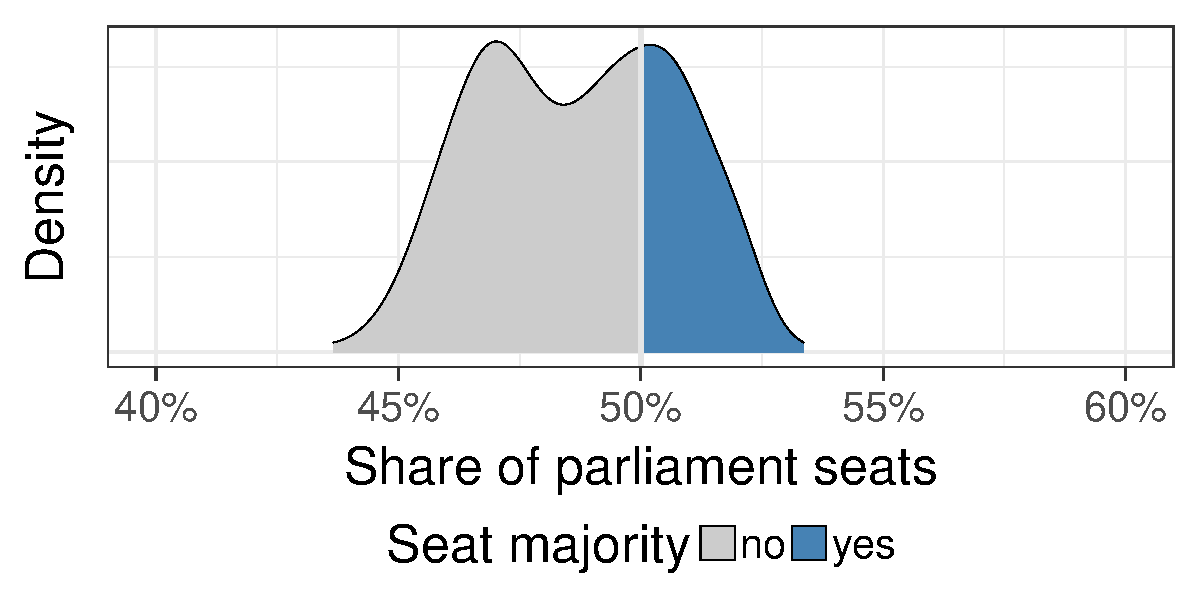
\includegraphics[width=0.45\textwidth]{figures/2013_forsa_cdufdp_lastPreelectionPoll.pdf}
\caption{Density of $10\,000$ simulated parliament seat shares for the coalition Union-FDP before the German federal election in September 2013 based on the Forsa opinion poll in Table \ref{tab_fdp}. The part of the density encoding for seat majorities is colored blue and resembles a probability of $26.33\%$.
\label{fig:seatDist}
}
\end{figure}

As such density plots depict both the probability and the underlying
uncertainty for specific coalitions, they are a nice possibility to communicate
uncertainty underlying opinion polls.

To visualize the {\it development} of such probabilities
%together with the underlying uncertainty
for a specific coalition we recommend extending the visualization of Figure \ref{fig:seatDist} by using ridgeline plots \citep{wilke_2017} for the simulated seat distributions. In Figure~\ref{fig:seatDist_time} this plot type and the development of majority probabilities is compared to
the redistributed raw shares, which are usually reported in media.

\begin{figure}[H]\centering
\begin{tabular}{ll}
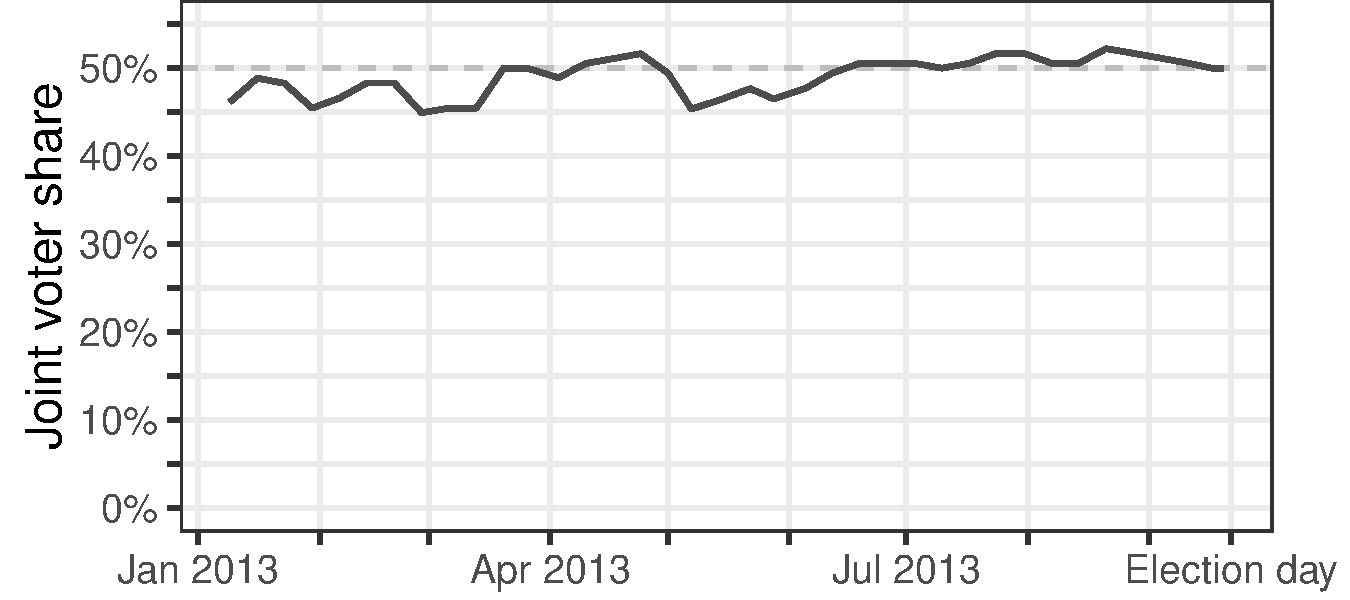
\includegraphics[height=.15\textwidth]{figures/2013_forsa_cdufdp_rawSharesRedist.pdf}
&
\multirow{2}{*}[13ex]{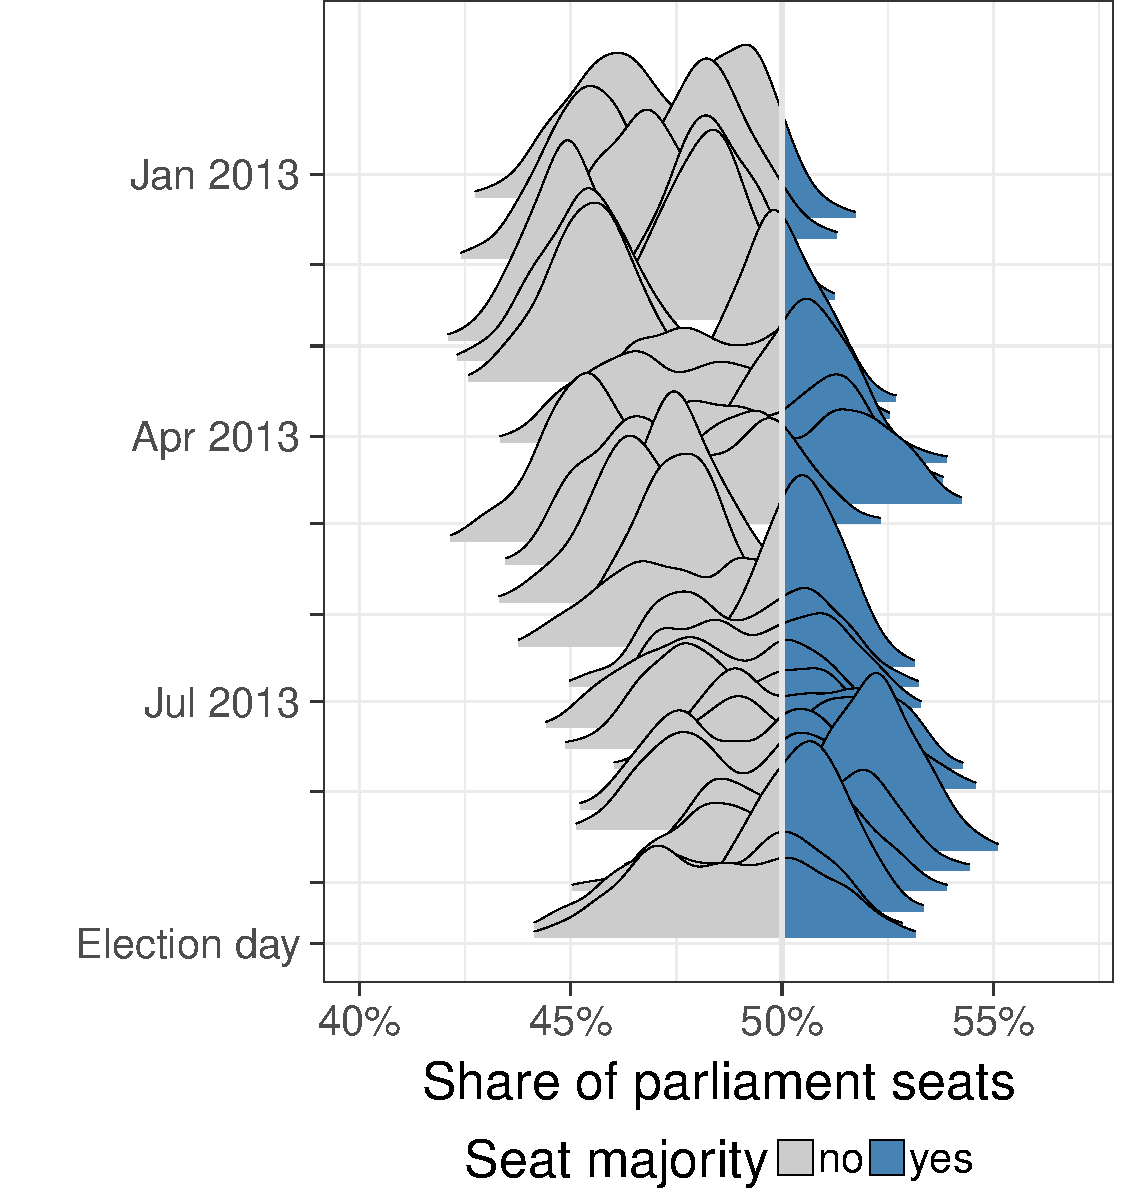
\includegraphics[height=30ex]{figures/2013_forsa_cdufdp_ridgeline.pdf}}
\\
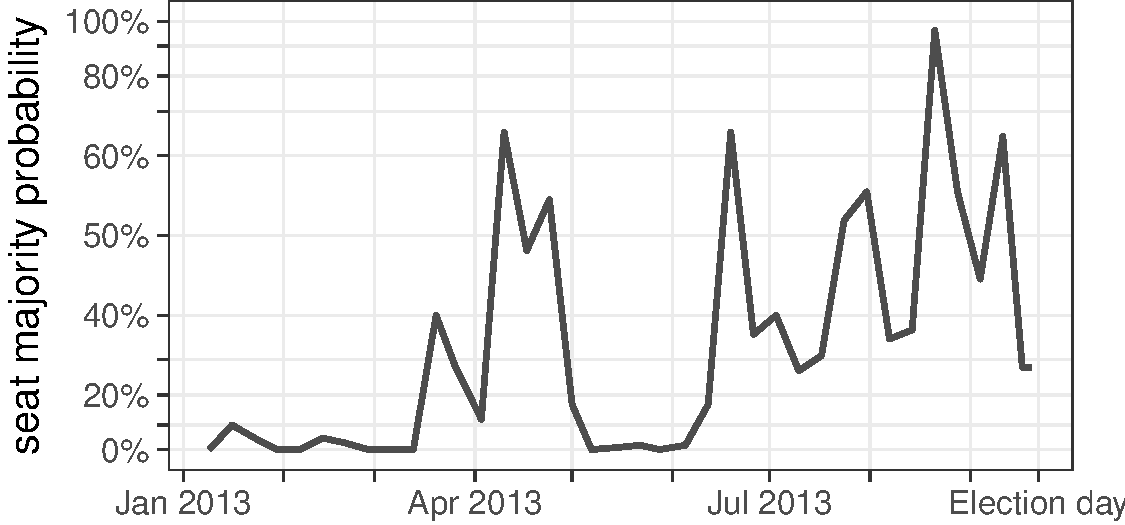
\includegraphics[height=.15\textwidth]{figures/2013_forsa_cdufdp_prob.pdf}
\end{tabular}
\caption{Development of the prospect to form a government of the coalition Union-FDP before the German federal election in September 2013 based on Forsa opinion polls.
Left top: Observed voter shares after redistribution. Left bottom: Probabilities to reach a majority of seats in parliament, based on $10\,000$ simulations. Right: Densities of simulated parliament seat shares based on $10\,000$ simulations. The parts of the densities encoding for seat majorities are colored blue.
\label{fig:seatDist_time}
}
\end{figure}

Comparing the redistributed voter shares and the seat majority probabilities
in Figure~\ref{fig:seatDist_time} it is clear that the probabilities contain
a lot more information than the voter shares. Especially, even small changes
in the redistributed voter share can make an immense difference regarding the
probability of the coalition to form a government.

To focus on the most relevant changes in the majority probabilities, we propose
the use of a skewed axis as shown in Figure~\ref{fig:seatDist_time}. In this axis
the range of values around $50\%$ is stretched and the range of values near
$0\%$ and $100\%$ is compressed. In this way, we put less weight on changes
where an event is {\it still highly (im)probable} and emphasize more relevant
changes after which an event gets more or less probable than $50\%$. Also,
consistently using another axis for the estimated probabilities prevents
confusion of probabilities and voter shares.



\section{Pooling approach} \label{sec:pooling}
In the presence of multiple published opinion polls, pooling is used to
summarize the observed results in order to reduce sample uncertainty.
To assure a reliable pooling regarding the current public opinion,
we only use polls published within the past 14 days and only use the
most recent survey published by each polling agency.

Looking at a single poll $i$, the observed number of votes $X_{ij}$ for each of $k$ parties follow a multinomial distribution with sample size $n_i$ and underlying, unknown party shares $\theta_j$ in the population.
% \begin{equation}
% X_{i1},\ldots, X_{ik} \sim Multinomial(n_i,\theta_1,\ldots,\theta_k).
% \end{equation}
Pooling over multiple such polls as independent random samples leads to another multinomial distribution for the summed number of votes $\sum_i X_{ij}$:
% Based on the multinomial distribution of the vote counts $X_{ij}$ of party $j$ in poll $i$ with underlying true party share $\theta_j$, pooling over multiple polls representing independent random samples would lead to a multinomial distribution for the summed number of votes $\sum_i X_{ij}$:
\begin{equation}
\sum\limits_i X_{i1},\ldots, \sum\limits_i X_{ik} \sim Multinomial \left( \sum\limits_i n_i,\theta_1,\ldots,\theta_k \right).
\end{equation}

Further analyses, however, showed that polls from different (German)
polling agencies are correlated
and the independency assumption does not hold.
Therefore, we adjust the resulting multinomial
distribution by using an \textit{effective sample size} \citep{hanley_2003},
reflecting that the aggregation over multiple polls does not contain 
information of a sample with $\sum_i n_i$ observations.

Quantification of pairwise correlation is done based on the variance of the
party share difference between two polls for a specific party.
The following equation holds for two independent
random sample polls $A$ and $B$:

\begin{equation}
\begin{aligned}
Var(X_A - X_B) &= Var(X_A) + Var(X_B) - 2 \cdot Cov(X_A, X_B) \\
\Leftrightarrow \ \ \ \ Cov(X_{Aj}, X_{Bj}) &= \frac{1}{2} \cdot \left(Var(X_{Aj}) + Var(X_{Bj}) - Var(X_{Aj} - X_{Bj}) \right).
\end{aligned}
\end{equation}

We take $Var(X_{Aj})$ and $Var(X_{Bj})$ as the theoretical variances of the binomially distributed, observed voter numbers and estimate $Var(X_{Aj} - X_{Bj})$ based on the observed differences between the party shares. Having done so, one can estimate the covariance $Cov(X_{Aj}, X_{Bj})$ and accordingly also the correlation. As the binomial variance is directly proportional to sample size, the effective sample size $n_{\text{eff}}$ can be defined as the ratio between the estimated variance of the pooled sample and the theoretical variance of a sample of size one:
$$
n_{\text{eff}} = \frac{Var(\text{pooled})}{Var(\text{sample of size 1})},
$$
with, in the case of two surveys,
$$
Var(\text{pooled}) = Var(X_A + X_B) = Var(X_A) + Var(X_B) + 2 Cov(X_A,X_B)
$$
and $Var(\text{sample of size 1})$ the theoretical variance of the pooled share.

Looking at the party-specific correlations between 20 surveys conducted by the two most regular German polling agencies, Emnid and Forsa, we on average end up with a medium high correlation, using mean party shares and sample sizes per institute for the theoretical variances. Other institute comparisons were not performed as too few published surveys were conducted that cover comparable time frames. For simplicity, we do not recalculate the correlation for each simulation, but rather set the correlation used in our methodology to $0.5$, i.e. a medium positive correlation.
For convenience, the calculation of $n_{\text{eff}}$ is based on the party with most votes, as the specific party choice only marginally affects the results.

In the case of two published polls with $1500$ and $2000$ respondents, respectively, and a pooled share of $40\%$
for the strongest party, the method leads
to an effective sample size of $n_{\text{eff}} = 2341$. Thus, the method reduces sample uncertainty
compared to using only single polls, but it is also quite conservative, compared to
assuming independence between the polls and using a summed sample size of $1500 + 2000 = 3500$.

As noted, in practice we use a timeframe of 14 days, i.e. all surveys published at maximum 14 days ago are included
in the calculation of the pooled sample. In the case of opinion polls for a specific election getting published
only very rarely one can also extend this timeframe, e.g. using the heuristics of including all surveys published up to 14 days
ago with weight 1 (using their true sample size), and all surveys within 15 to 28 days age with halved weight
(using the halved sample size).



\section{Application} \label{sec:application}
As previously mentioned, (an earlier iteration of) our method entered
general media reporting about opinion polls before the German federal elections
2013 and 2017 \citep[cf.][]{wahlistik_2013, gelitz_2017}.
We will in the following revise the polling situation before these two elections
to underline the differences between standard media reporting on election polls
-- focusing on the interpretation of the raw or redistributed observed shares --
and our approach based on estimated probabilities.

For each of the two elections we base the discussion on opinion polls published
by major German polling agencies (i.e. Allensbach, Emnid, Forsa, Forschungsgruppe Wahlen,
GMS, Infratest dimap and INSA), starting one year before each election.
Opinion poll data from these polling agencies is publicly available
on \texttt{www.wahlrecht.de}. The polls are pooled using a time window
of 14 days. For the estimation of event probabilities $10\,000$ simulations
were used.


\subsection{German federal election 2013} \label{subsec:2013}
In the legislative period from 2009 to 2013, the German government was formed by
a coalition of the conservatives (Union) and the liberals (FDP).
Main interest before the election on September 22nd, 2013 was in whether the
coalition could sustain its majority of parliament seats. A key role thereby played the FDP,
which had to successfully pass into parliament -- i.e. achieve at least the
minimum voter share of $5\%$ -- for a success of the coalition.

\begin{figure}[H]\centering
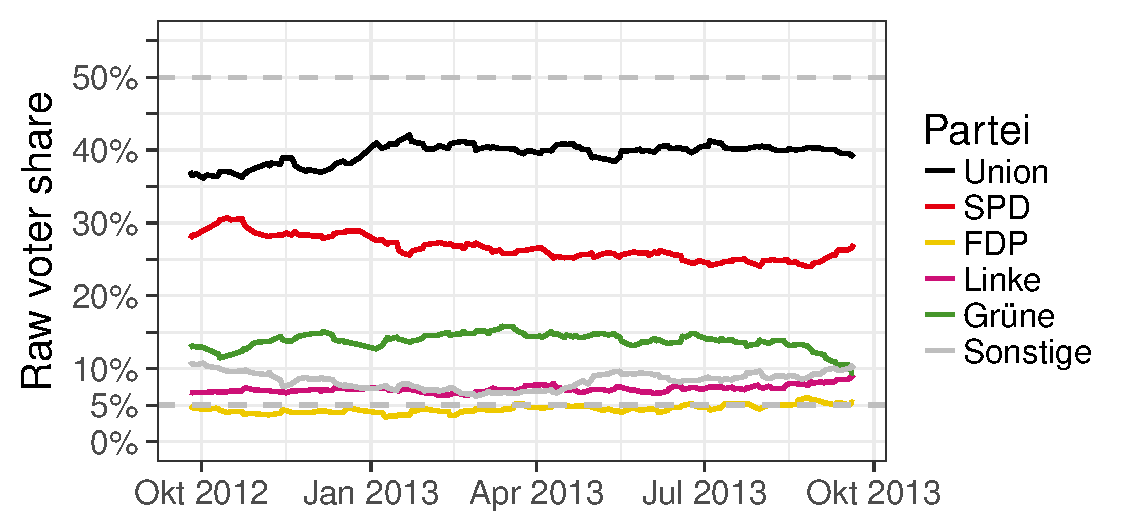
\includegraphics[width=0.6\textwidth]{figures/2013_pooled_rawShares.pdf}
\caption{Development of the pooled raw voter shares from October 2012 until election day on September 22nd, 2013, based on a pooling window of 14 days.
As specific voter shares for AfD were only sparsely reported before the election in 2013 the party is contained in ''Others''.
\label{fig:2013}
}
\end{figure}


\paragraph{FDP passing the 5\% hurdle} \ \\
The poll-based prospect of FDP to successfully pass into parliament is visualized
in Figure~\ref{fig:2013_fdp}.
As can be seen, the raw voter share of the party only exceeded the necessary share
of $5\%$ over short periods of time and only once reached a maximum value
of $6\%$ (top left pane in Fig.~\ref{fig:2013_fdp}). Similarly, the probability
for the party to pass the hurdle only rarely rose over $50\%$ (bottom left pane). 
However, beginning
from the end of August 2013 until election day, the pooled voter shares and the
corresponding probabilities consitently lay over $5\%$ and $50\%$, respectively,
stating that -- shortly before election day -- a success of the FDP was more
probable than a failure.

Comparing voter shares and probabilities, Figure~\ref{fig:2013_fdp} shows
that small changes in the overall share of a party can dramatically influence
event probabilities, depending on the base level of the voter share and 
-- in this example -- its closeness to the $5\%$ hurdle.
In this regard, probabilities make it easier to deduce {\it relevant} information
from election polls as they incorporate both the closeness of the observed shares
to the relevant threshold and sample uncertainty.
E.g., the probability corresponding to voter shares of $4\%$ and $6\%$ correspond to
very definite probabilities of near $0\%$ and $100\%$, respectively,
and communicating such probabilities leads to a way clearer perception of
the current public opinion than does the reporting of FDP voter share and sample size only.

\begin{figure}[H]\centering
\begin{tabular}{ll}
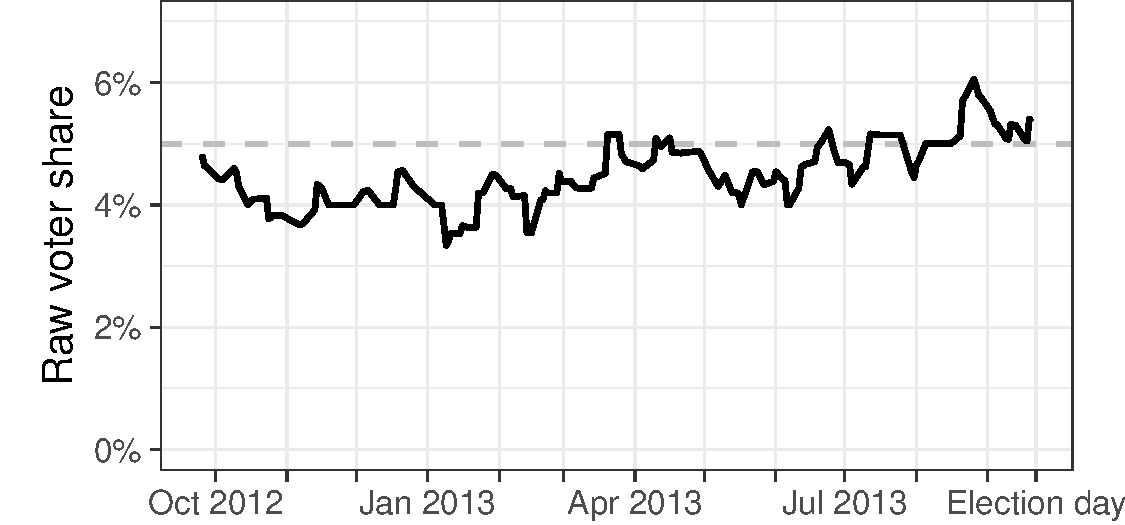
\includegraphics[height=.15\textwidth]{figures/2013_pooled_fdp_rawShares.pdf}
&
\multirow{2}{*}[13ex]{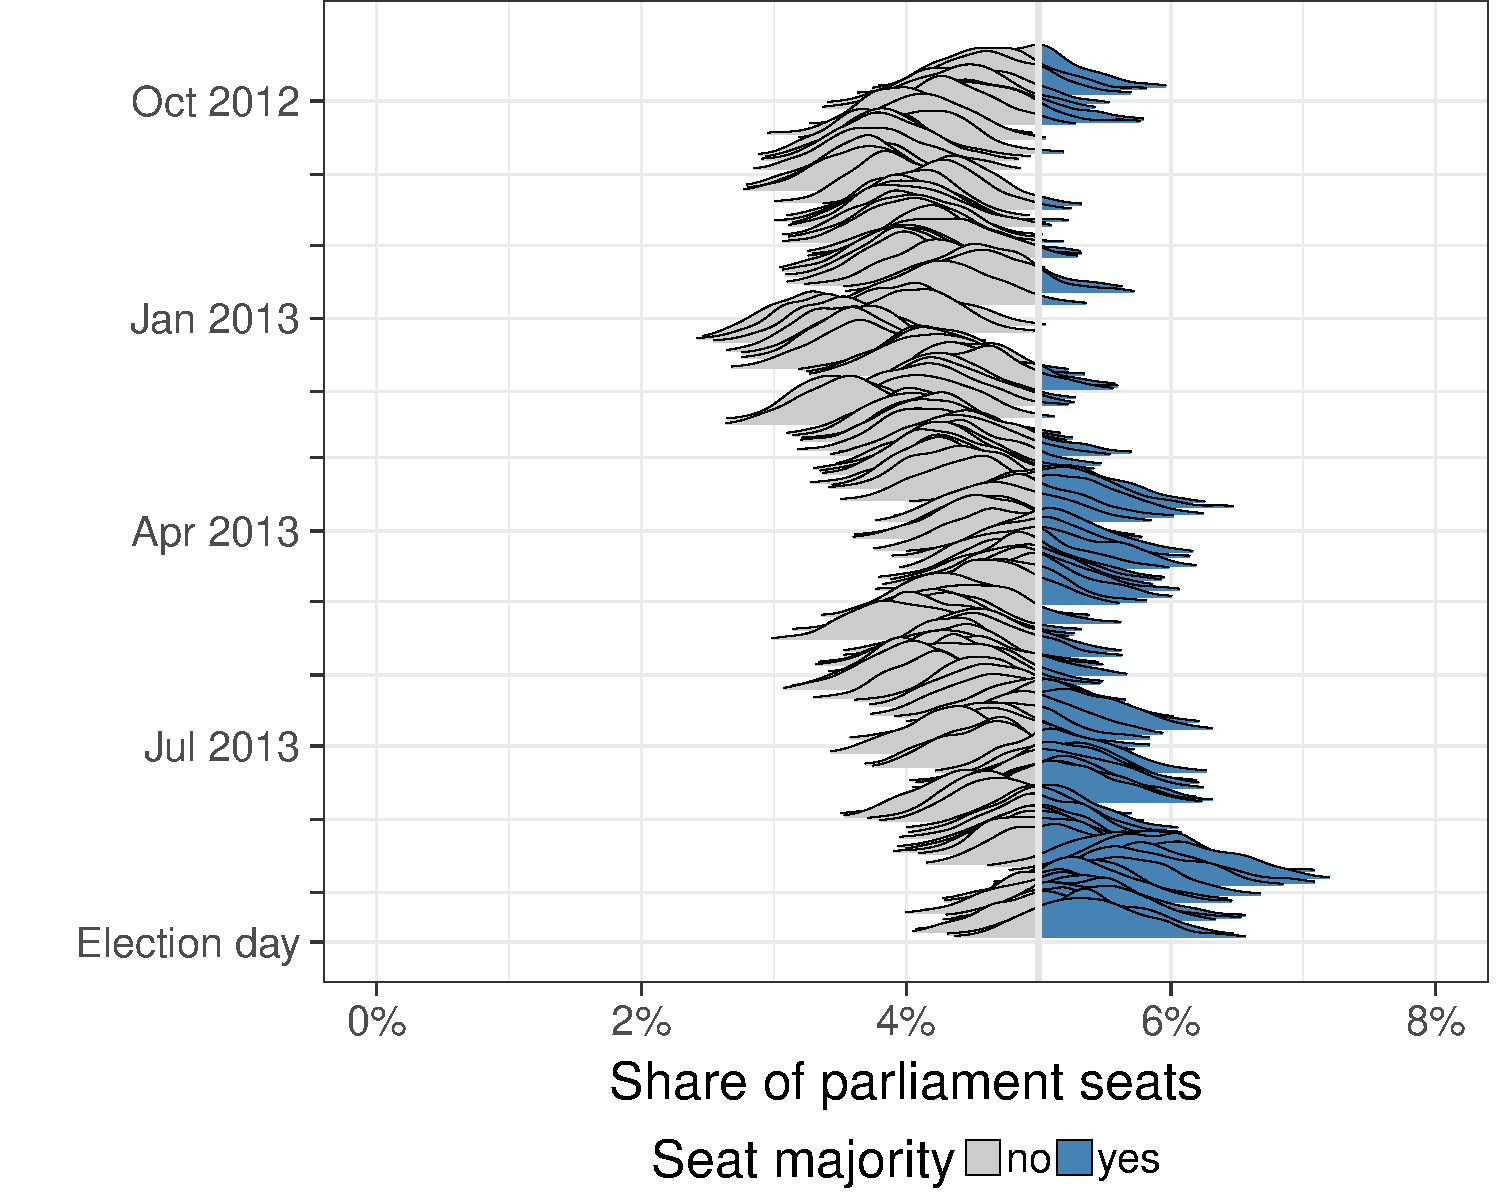
\includegraphics[height=30ex]{figures/2013_pooled_fdp_ridgeline.pdf}}
\\
\includegraphics[height=.15\textwidth]{figures/2013_pooled_fdp_passingProb.pdf}
\end{tabular}
\caption{Development of the prospect of FDP to pass the $5\%$ hurdle before the German federal election in September 2013 based on pooled opinion polls.
Left top: Observed voter shares before redistribution. Left bottom: Probabilities to pass the $5\%$ hurdle, based on $10\,000$ simulations. Right: Densities of simulated raw voter shares based on $10\,000$ simulations. The parts of the densities encoding for successfully possing the hurdle are colored blue.
\label{fig:2013_fdp}
}
\end{figure}


\paragraph{Union-FDP coalition majority} \ \\
Figure \ref{fig:2013_cdufdp} visualizes the pooled opinion poll results
for the potential coalition Union-FDP.
Starting from a redistributed voter share of around $43\%$ in October 2012,
the voter share rose steadily, reaching its maximum
of ca. $51\%$ about one month before election day.

Only taking this development of the redistributed voter shares into
consideration, one would conclude that -- apart from a short
time window in August/September of 2013 -- a majority of the Union-FDP
coalition would be slightly missed if the election would have been held.
In the best case, sample uncertainty would be reported, making
a majority for the coalition {\it (highly) improbable}. A more
solid quantification of uncertainty however is not given.

\begin{figure}[H]\centering
\begin{tabular}{ll}
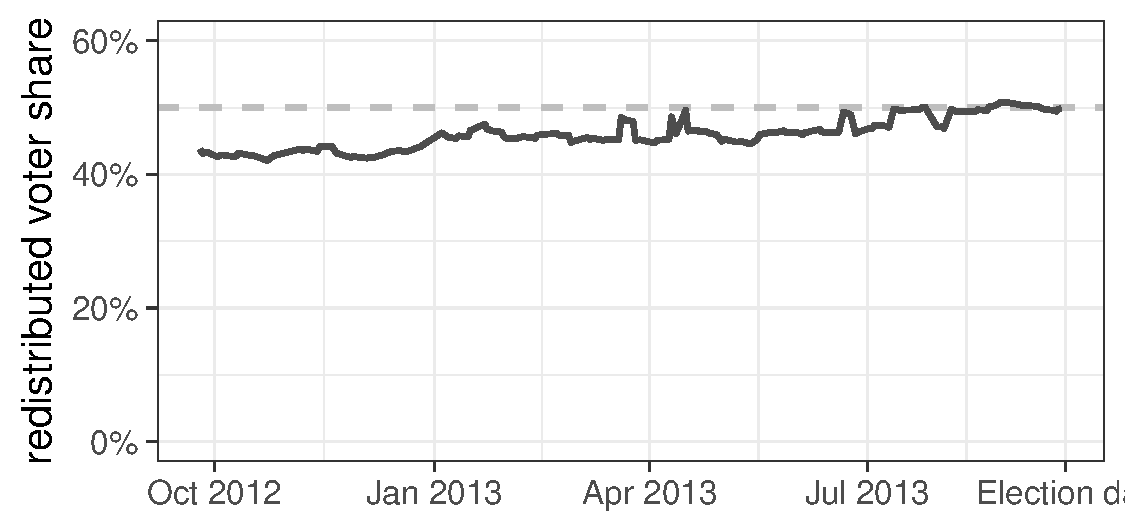
\includegraphics[height=.15\textwidth]{figures/2013_pooled_cdufdp_rawSharesRedist.pdf}
&
\multirow{2}{*}[13ex]{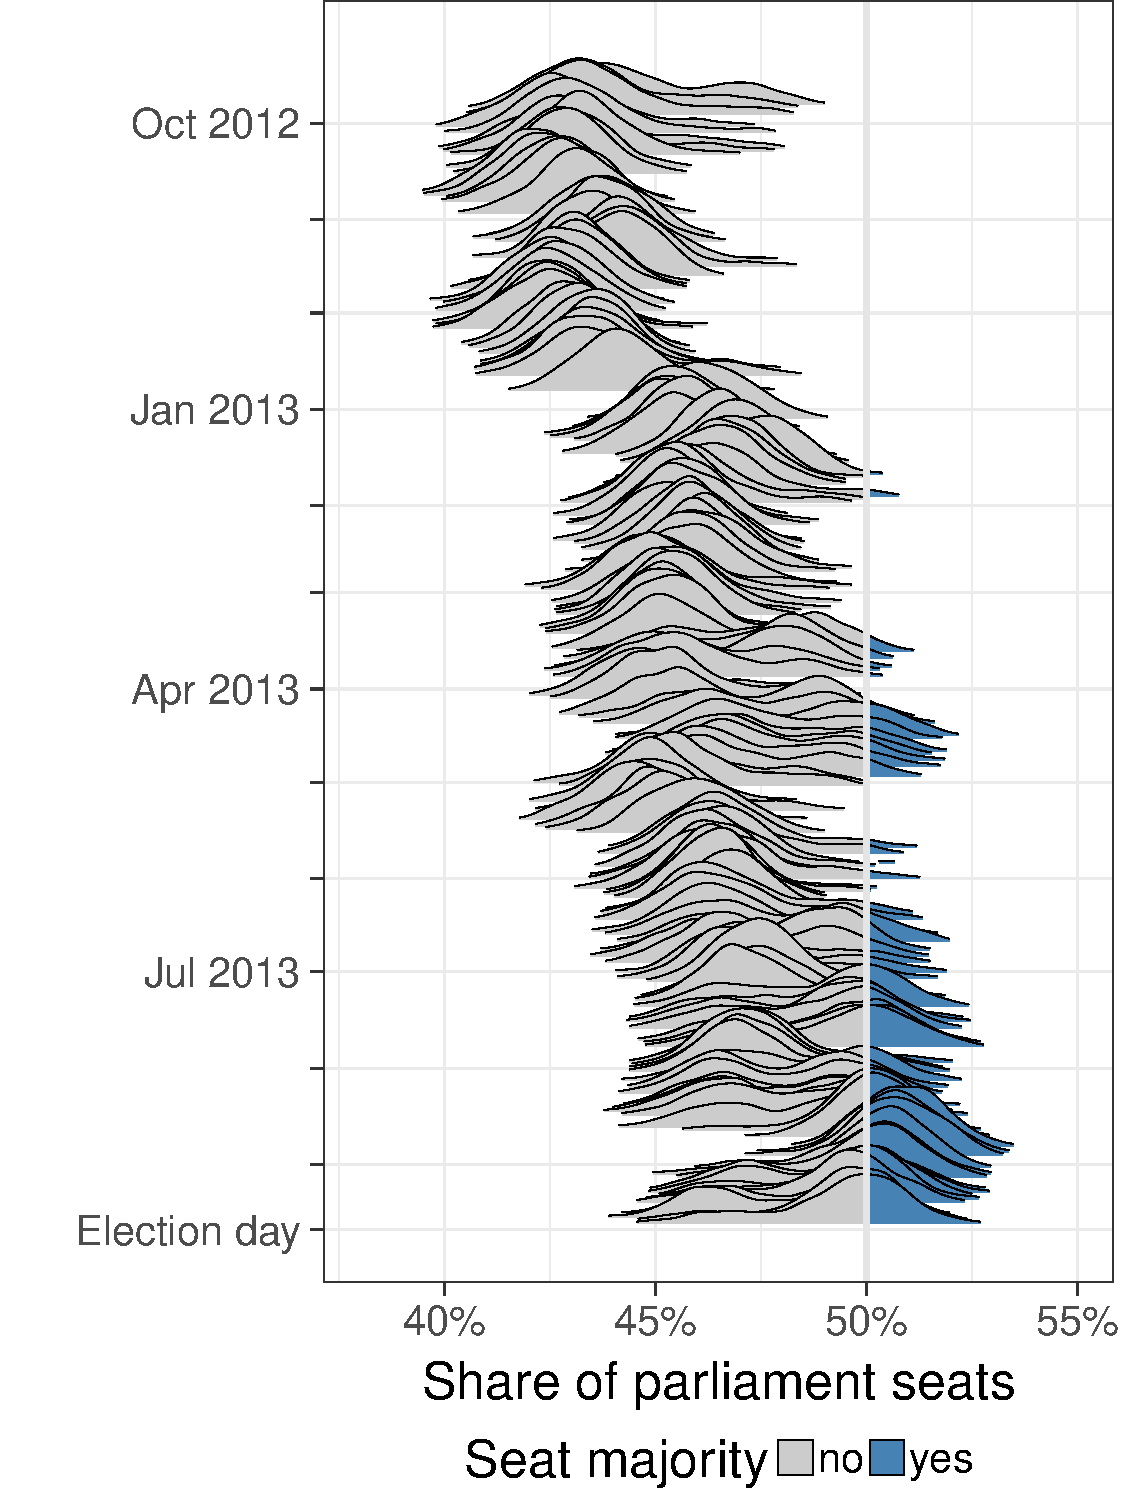
\includegraphics[height=.3\textwidth]{figures/2013_pooled_cdufdp_ridgeline.pdf}}
\\
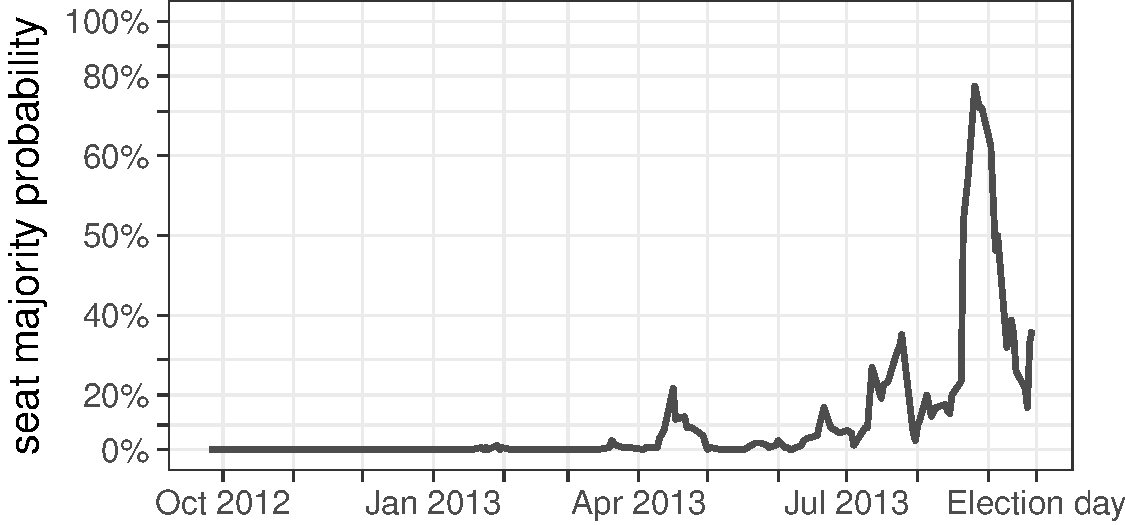
\includegraphics[height=.15\textwidth]{figures/2013_pooled_cdufdp_prob.pdf}
\end{tabular}
\caption{Development of the prospect to form a government of the coalition Union-FDP before the German federal election in September 2013 based on pooled opinion polls.
Left top: Observed voter shares after redistribution. Left bottom: Probabilities to reach a majority of seats in parliament, based on $10\,000$ simulations. Right: Densities of simulated parliament seat shares based on $10\,000$ simulations. The parts of the densities encoding for seat majorities are colored blue.
\label{fig:2013_cdufdp}
}
\end{figure}

Looking at the estimated seat majority probabilities together with
the simulated seat share densities instead draws a more comprehensive picture
of the situation.
While the overall development of probabilities has the same structure
as the redistributed voter shares, i.e. they rose with time,
there are two points that clearly get more weight when shifting 
the focus in reporting towards discussing {\it how probable} events are:
First of all, the impact of small changes in voter shares is nicely resembled
in the probability development. As is the case for the FDP prospect in Figure~\ref{fig:2013_fdp},
how big the {\it relevant} impact of a change in voter share on event
probabilities is depends heavily on the base level of the voter share.
E.g., a rise in voter share from $45\%$ to $48\%$ in March 2013 only had a very small impact on 
the absolute probability, as a seat majority is still very improbable based on a share of $48\%$.
Instead, even very small changes near a voter share of $50\%$ heavily influence the event probabilities.
Second of all, probabilities do not only take the summed party
shares and their general uncertainty into account,
but also implicitly cover the 
uncertainty regarding whether FDP passes the $5\%$ hurdle
or not. Apart from the end of August 2013, the latter event 
is highly uncertain and thus overall majority probabilities of
the coalition are comparatively small, even for pooled voter shares around $50\%$.
The inclusion of the FDP-based uncertainty is nicely visualized in the
ridgeline plot (right panel in Fig.~\ref{fig:2013_cdufdp}), where
the densities are bimodal or unimodal depending on whether the raw FDP voter share
is close to $5\%$ or not (see Fig.~\ref{fig:2013_fdp}), respectively.



\subsection{German federal election 2017} \label{subsec:2017}
After the federal election in 2013, none of the desired coalitions
reached a seat majority
and a grand coalition between Union and the social democratic SPD
became the government from 2013 to 2017.
The goal of both Union and SPD for the election on September 24th, 2017
was to achieve a majority with a coalition apart from the grand coalition
and thus there were multiple coalitions of interest before the election.
In this regard, we will focus on the most prominent Union-led coalition,
i.e. again Union-FDP, and the most prominent SPD-led coalition,
i.e. a union of SPD, the Left and the Greens, which was
-- based on the joint voter share -- the strongest alternative to a Union-led
government and was not clearly denied by the member parties until several weeks
before election day.
Also, after the rise of the right-wing party AfD major interest was
in whether this party that in 2013 slightly missed the $5\%$ hurdle
would become the third strongest party in parliament after Union and SPD.
The pooled poll results before the 2017 election are shown in Figure~\ref{fig:2017}.

\begin{figure}[H]\centering
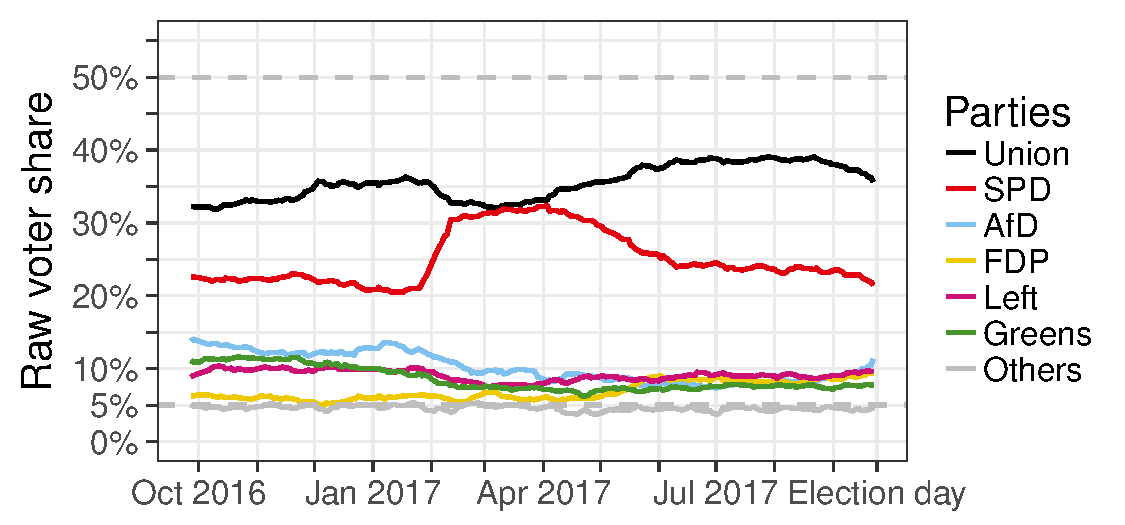
\includegraphics[width=0.6\textwidth]{figures/2017_pooled_rawShares.pdf}
\caption{Development of the pooled raw voter shares from October 2016 until election day on September 24nd, 2017, based on a pooling window of 14 days.
\label{fig:2017}
}
\end{figure}


\paragraph{Union-FDP coalition majority} \ \\
Compared to the federal election 2013, the situation for a
coalition between Union and FDP before the election in 2017 
was quite different as FDP voter shares were at most times
clearly above the $5\%$ hurdle (see Fig.~\ref{fig:2017}).
However, as the share of Union was lower than in 2013,
the joint redistributed voter share shortly before election day
was at no moment bigger than $50\%$.
As can be seen in Figure~\ref{fig:2017_cdufdp}, the coalition had
a poll-based redistributed share of around $40\%$ in october 2016
and reached its maximum share of nearly $49.8\%$ about one month
before election day.
Again, interpreting only the observed redistributed voter shares
is hard for the general public as no easily accessible quantification 
of uncertainty is given.

Especially as of the rising voter shares starting in February 2017,
an interesting question is which voter share is necessary to have
a relevant prospect to gain seat majority and which voter shares
encode for an irrelevantly small majority probability, based on the
(pooled) sample sizes.
Regarding the latter, the ridgeline plot in Figure~\ref{fig:2017_cdufdp}
shows that parliament seat shares (or correspondingly voter shares)
below around $47.5\%$ correspond to negligibly small success probabilities of $<1\%$,
based on pooled effective sample sizes of around 3000.
On the other hand, based on comparable sample sizes,
observed shares of $49\%$ and $49.5\%$
corresponded to probabilities of around $14\%$ and $25\%$, respectively.

Overall, one month before election day the coalition had a good prospect
on winning the election based on a redistributed share of $49.8\%$ and
a probability of nearly $40\%$.
However, until two days before the election the pooled share and the probability
dropped again to $47.4\%$ and $0.4\%$, respectively, making a success
of the two parties highly improbable.

\begin{figure}[H]\centering
\begin{tabular}{ll}
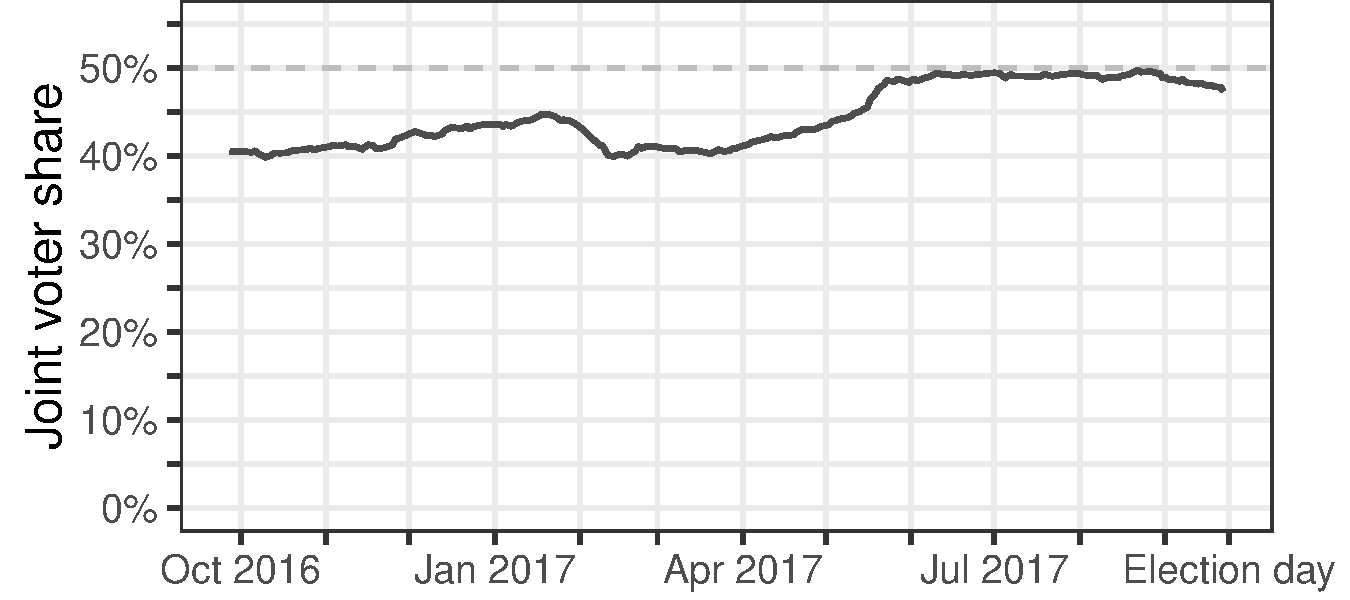
\includegraphics[height=.15\textwidth]{figures/2017_pooled_cdufdp_rawSharesRedist.pdf}
&
\multirow{2}{*}[13ex]{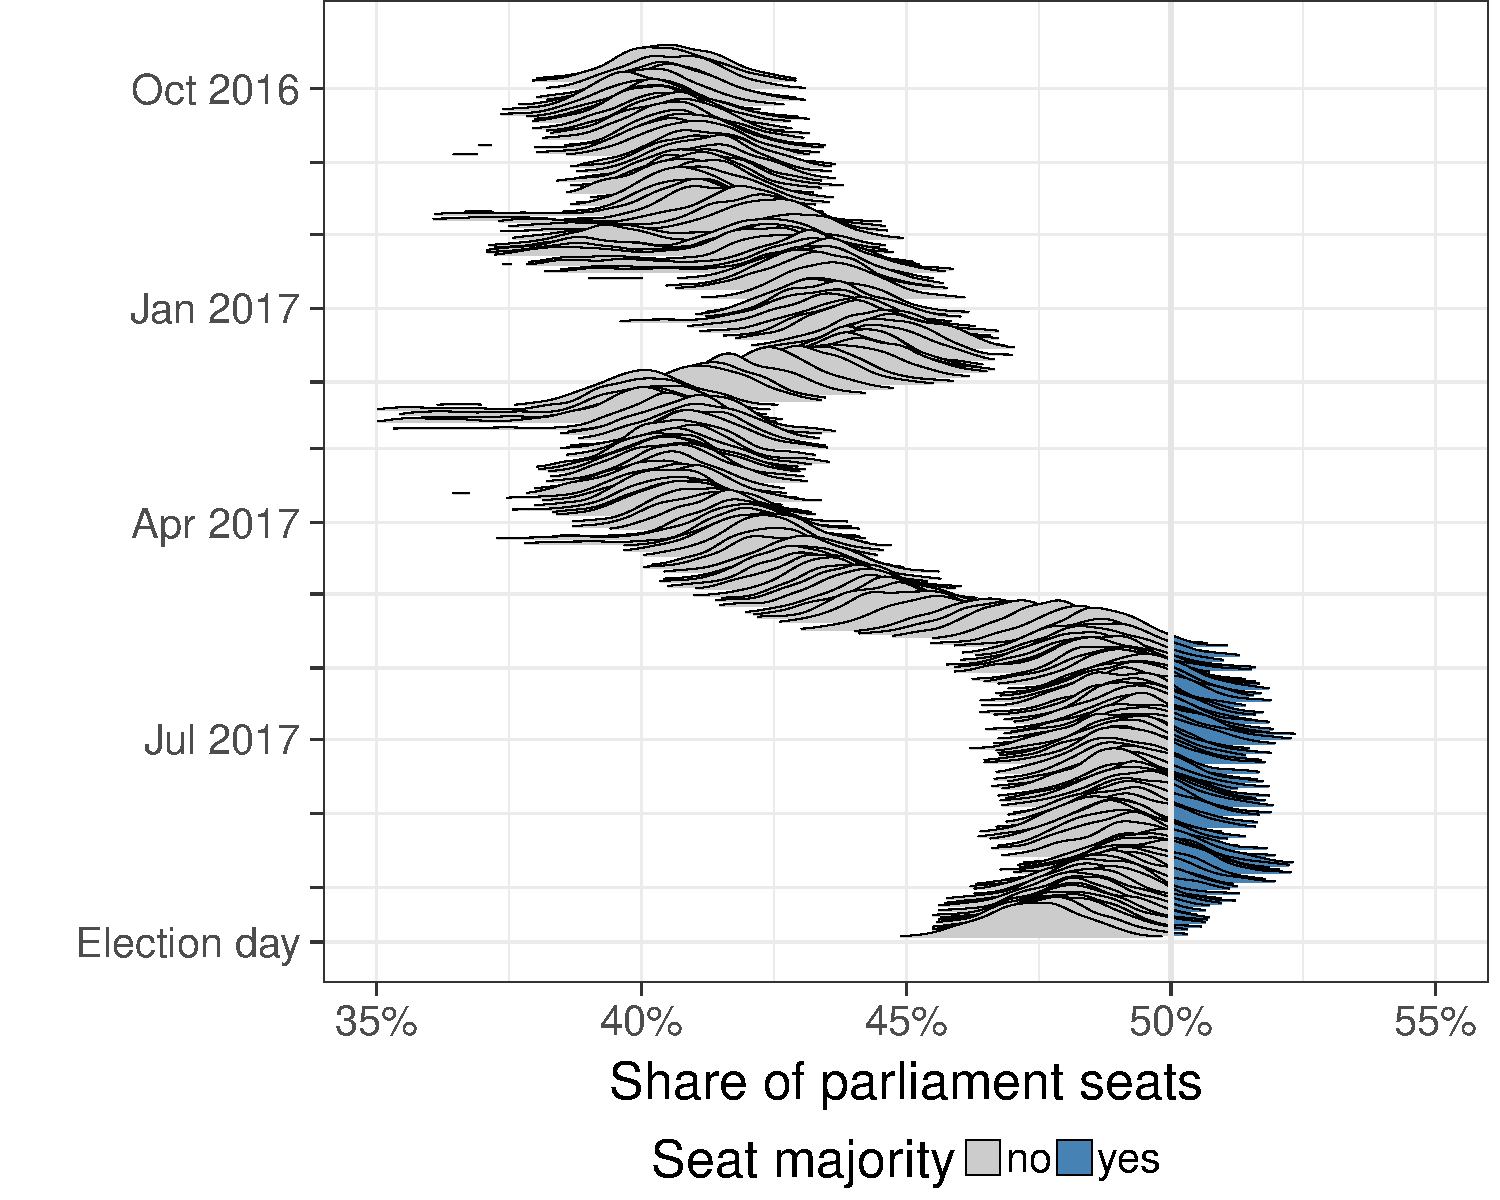
\includegraphics[height=30ex]{figures/2017_pooled_cdufdp_ridgeline.pdf}}
\\
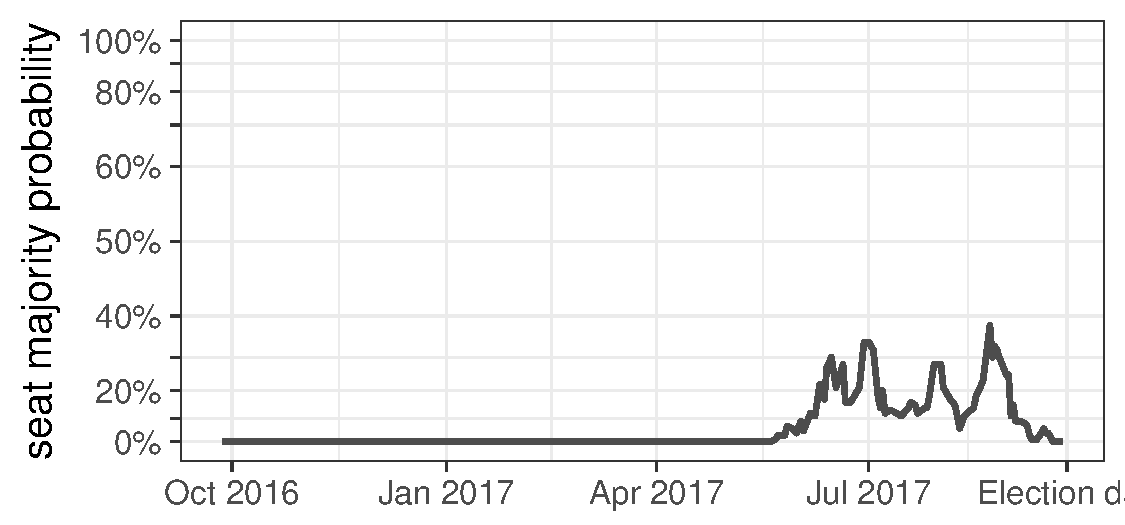
\includegraphics[height=.15\textwidth]{figures/2017_pooled_cdufdp_prob.pdf}
\end{tabular}
\caption{Development of the prospect to form a government of the coalition Union-FDP before the German federal election in September 2017 based on pooled opinion polls.
Left top: Observed voter shares after redistribution. Left bottom: Probabilities to reach a majority of seats in parliament, based on $10\,000$ simulations. Right: Densities of simulated parliament seat shares based on $10\,000$ simulations. The parts of the densities encoding for seat majorities are colored blue.
\label{fig:2017_cdufdp}
}
\end{figure}


\paragraph{SPD-Left-Greens coalition majority} \ \\
Regarding the voter share development of SPD, the year before 
the federal election in 2017 was shaped by an extreme uprise starting
in the end of January 2017 when Martin Schulz was elected to be the SPD chancellor
candidate and a subsequent, steady decline from April 2017 on (see Fig.~\ref{fig:2017}).
Accordingly, the coalition between SPD, the Left and the Greens had
their best poll results between February and May 2017 as is shown in Figure~\ref{fig:2017_spdleftgreens}.
The maximum share was reached in April with a redistributed voter
share of $50.04\%$, which corresponded to a probability of obtaining the
parliament seat majority of $47.8\%$.
Starting in April, the probability again dropped to negligibly small values.
Shortly before election day, the joint share
reached a value of around $41\%$ and a success at the election wasn't even
slightly possible.

As a special note, the ridgeline plot in Figure~\ref{fig:2017_spdleftgreens}
again nicely visualizes the uncertainty underlying the event of
interest. This is not only limited to parties forming the potential coalition,
but also includes information about all other causes of uncertainty in the data.
E.g., in November and December of 2016, the seat share distribution clearly
is bimodal as in a relevant share of simulations FDP does not pass
the $5\%$ hurdle and more votes are redistributed in these cases.

\begin{figure}[H]\centering
\begin{tabular}{ll}
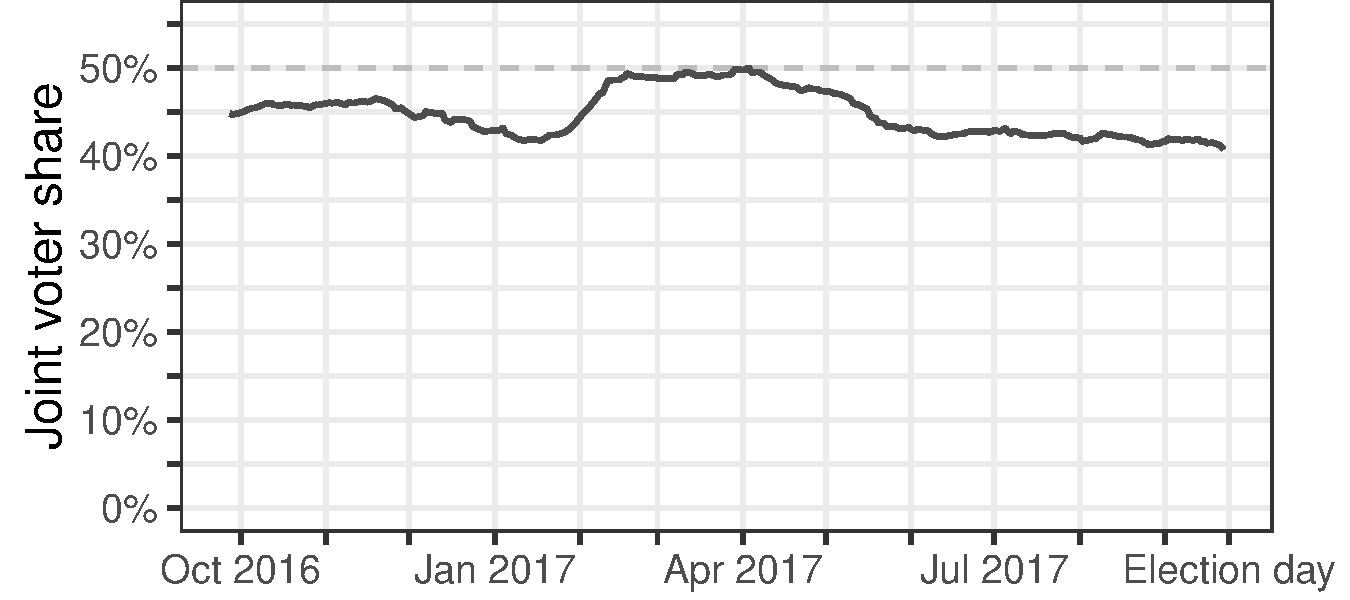
\includegraphics[height=.15\textwidth]{figures/2017_pooled_spdleftgreens_rawSharesRedist.pdf}
&
\multirow{2}{*}[13ex]{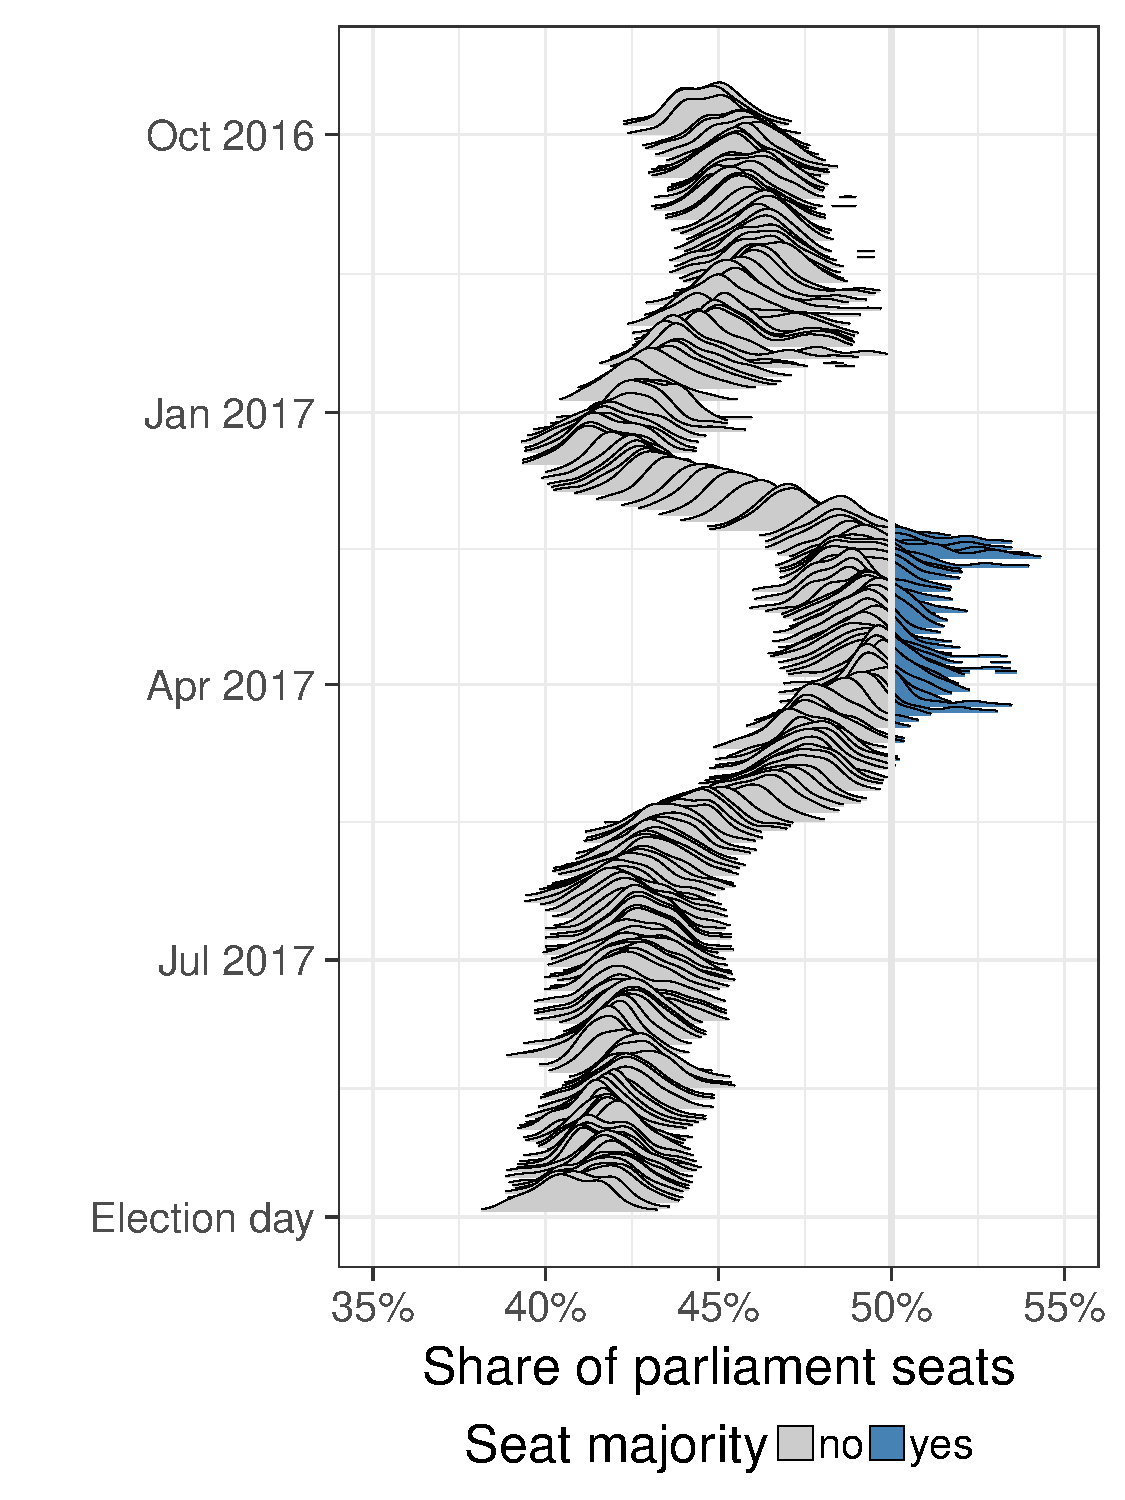
\includegraphics[height=30ex]{figures/2017_pooled_spdleftgreens_ridgeline.pdf}}
\\
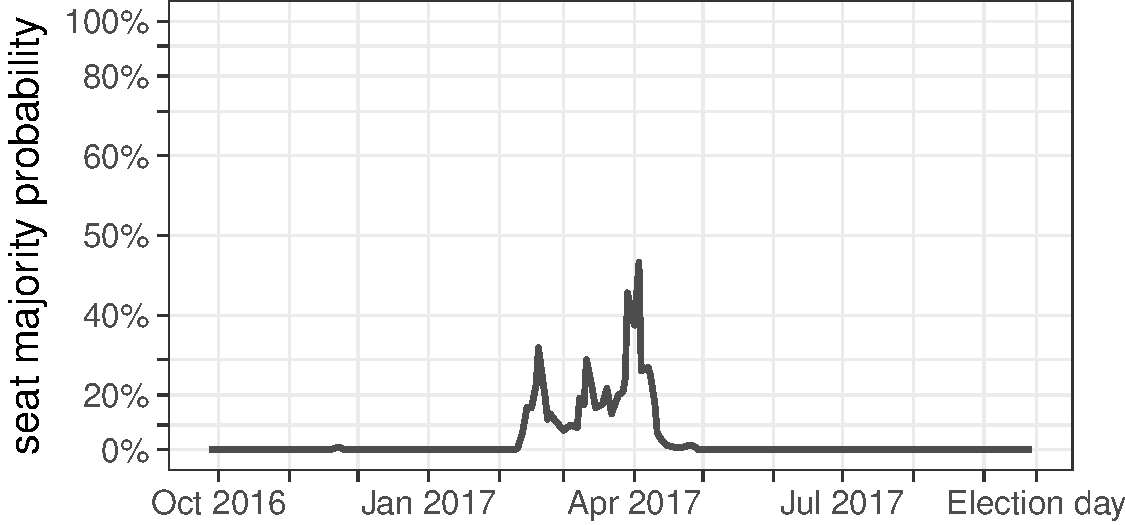
\includegraphics[height=.15\textwidth]{figures/2017_pooled_spdleftgreens_prob.pdf}
\end{tabular}
\caption{Development of the prospect to form a government of the coalition SPD-Left-Greens before the German federal election in September 2017 based on pooled opinion polls.
Left top: Observed voter shares after redistribution. Left bottom: Probabilities to reach a majority of seats in parliament, based on $10\,000$ simulations. Right: Densities of simulated parliament seat shares based on $10\,000$ simulations. The parts of the densities encoding for seat majorities are colored blue.
\label{fig:2017_spdleftgreens}
}
\end{figure}


\paragraph{AfD becoming third strongest party} \ \\
Special interest in the election was on which party would
get the third best result after the major parties Union and SPD.
With observed voter shares of at most times over $8\%$,
the right-wing AfD had a very good prospect to become a member
of the German parliament for the first time (see Fig.~\ref{fig:2017_afd}).
Using our KOALA approach it is easily possible to estimate probabilities
for the event that AfD becomes third strongest party in parliament,
summarizing this complex issue with several parties involved into one
development of probabilities.

During the year before the federal election in 2017, the polling situation
regarding AfD underwent heavy changes. The party in January 2017 had a $3.9\%$ lead
over Left and Greens (corresponding to an estimated probability of $100\%$), 
dropped to being $1.9\%$ behind the Left in June ($1.2\%$)
and rose back to a $1.7\%$ lead over the Left and FDP shortly before election
day ($96.8\%$).

Again, reporting probabilities instead of multiple raw voter shares
for the multiple parties allows for a much clearer communication of the
uncertainty underlying the situation, especially by breaking the matter down
to simple probabilities instead of one having to compare multiple party
shares on one's own.

\begin{figure}[H]\centering
\begin{tabular}{l}
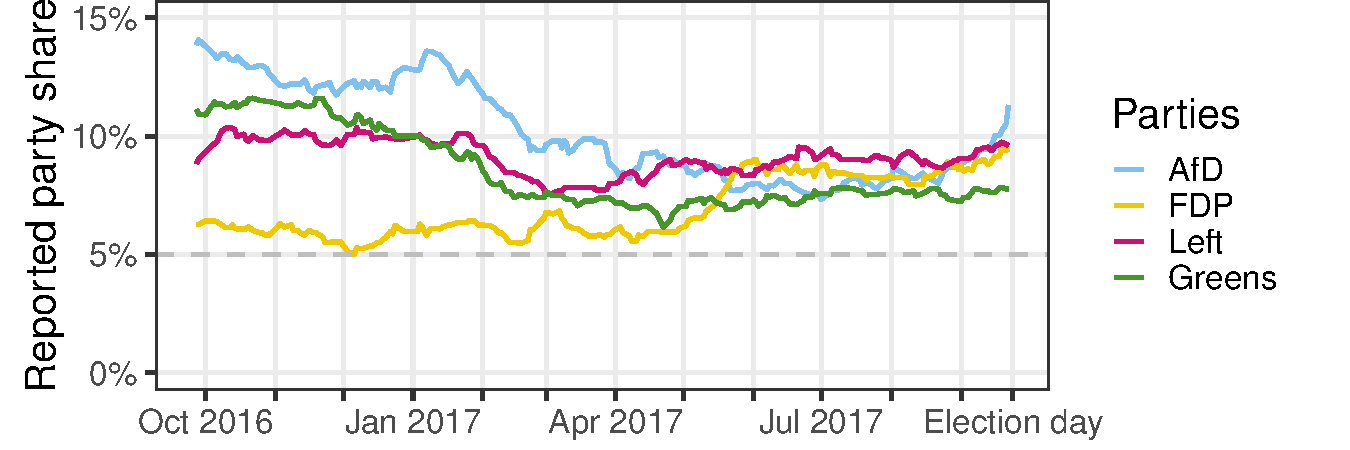
\includegraphics[height=.2\textwidth]{figures/2017_pooled_afd_rawShares.pdf}
\\
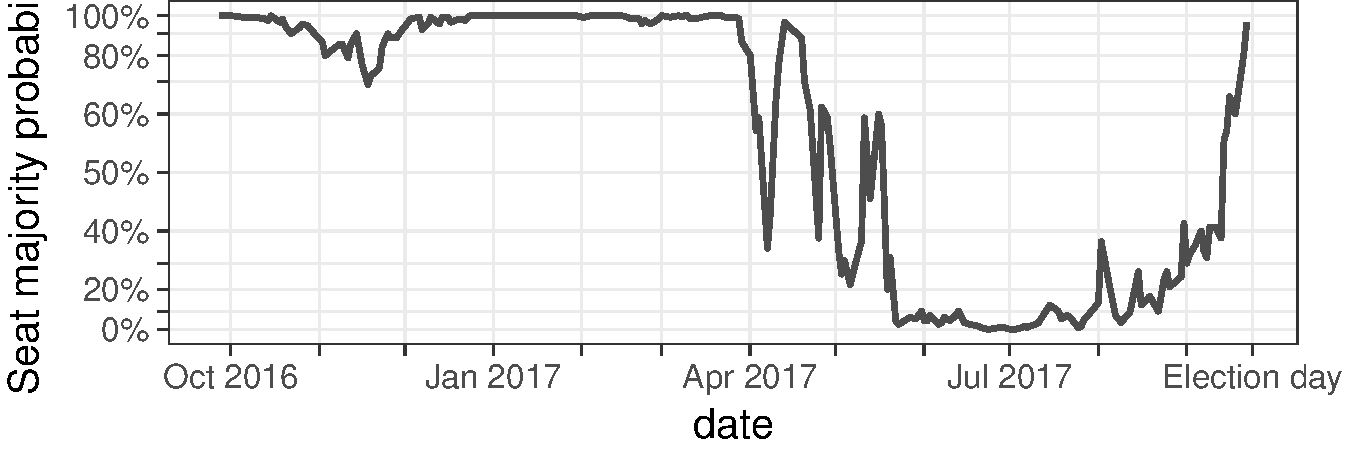
\includegraphics[height=.15\textwidth]{figures/2017_pooled_afd_thirdPartyProb.pdf}
\end{tabular}
\caption{Development of the prospect of AfD to become the third strongest party before the German federal election in September 2017 based on pooled opinion polls.
Left top: Observed voter shares before redistribution. Left bottom: Probabilities to become third strongest party, based on $10\,000$ simulations.
\label{fig:2017_afd}
}
\end{figure}


\section{Conclusion} \label{sec:conclusion}
We presented the KOALA (Coalition analysis) approach,
i.e. a Bayesian, Monte Carlo based method to estimate probabilities of specific 
election outcomes based on publicly available opinion polls.
A pooling approach allows for the inclusion of information from multiple
surveys and reduces sample uncertainty.
The estimated event probabilities are easy to communicate to the general
public and prevent improper poll-based reporting as they include 
sample uncertainty in a natural way.
We visualize the results on a publicly available website for chosen elections and
provide the open-source \texttt{R} package \texttt{coalitions} that allows for a
straightforward application of the method to any multi-party electoral system.
In this manner, our long-term goal is to make proper uncertainty assessment
in general opinion poll-based reporting the rule, rather than an exception.



% % For one-column wide figures use
% \begin{figure}
% % Use the relevant command to insert your figure file.
% % For example, with the graphicx package use
%   \includegraphics{figures/seatDist_ridgeline.pdf}
% % figure caption is below the figure
% \caption{Please write your figure caption here}
% \label{fig:1}       % Give a unique label
% \end{figure}
% %
% % For two-column wide figures use
% \begin{figure*}
% % Use the relevant command to insert your figure file.
% % For example, with the graphicx package use
%   \includegraphics[width=0.75\textwidth]{figures/seatDist_ridgeline.pdf}
% % figure caption is below the figure
% \caption{Please write your figure caption here}
% \label{fig:2}       % Give a unique label
% \end{figure*}
%
% % For tables use
% \begin{table}
% % table caption is above the table
% \caption{Please write your table caption here}
% \label{tab:1}       % Give a unique label
% % For LaTeX tables use
% \begin{tabular}{lll}
% \hline\noalign{\smallskip}
% first & second & third  \\
% \noalign{\smallskip}\hline\noalign{\smallskip}
% number & number & number \\
% number & number & number \\
% \noalign{\smallskip}\hline
% \end{tabular}
% \end{table}


%\begin{acknowledgements}
%If you'd like to thank anyone, place your comments here
%and remove the percent signs.
%\end{acknowledgements}

% BibTeX users please use one of
% \bibliographystyle{spbasic}      % basic style, author-year citations
%\bibliographystyle{spmpsci}      % mathematics and physical sciences
%\bibliographystyle{spphys}       % APS-like style for physics
\bibliography{bauer_2018}   % name your BibTeX data base

% Non-BibTeX users please use
% \begin{thebibliography}{}
%
% and use \bibitem to create references. Consult the Instructions
% for authors for reference list style.
%
% \bibitem{RefJ}
% % Format for Journal Reference
% Author, Article title, Journal, Volume, page numbers (year)
% % Format for books
% \bibitem{RefB}
% Author, Book title, page numbers. Publisher, place (year)
% % etc
% \end{thebibliography}

\end{document}
% end of file template.tex

